\documentclass[11pt]{article}

\usepackage[letterpaper,margin=1in]{geometry}
\usepackage[T1]{fontenc}
\usepackage{lmodern}
\usepackage{microtype}
\usepackage{amsmath,amssymb,mathtools}
\usepackage{booktabs}
\usepackage{array}
\usepackage{enumitem}
\usepackage{xcolor}
\usepackage{tikz}
\usetikzlibrary{arrows.meta,positioning,calc,patterns}
\usepackage{pgfplots}
\pgfplotsset{compat=1.18}
\usepackage{tocloft}
\usepackage{hyperref}
\usepackage{cleveref}
\usepackage{fancyhdr}

\definecolor{deepblue}{RGB}{36,76,120}
\definecolor{softgreen}{RGB}{228,241,224}
\definecolor{softred}{RGB}{250,229,225}
\definecolor{softblue}{RGB}{228,238,249}
\definecolor{softgray}{RGB}{245,245,245}
\definecolor{accent}{RGB}{125,45,45}

\hypersetup{
  colorlinks=true,
  linkcolor=deepblue,
  citecolor=deepblue,
  urlcolor=deepblue,
  pdftitle={Why Zero-Centered Hidden Activations Help Gradient Descent},
  pdfauthor={Paul Agron}
}

\setlength{\parindent}{0pt}
\setlength{\parskip}{0.65em}
\setlist[itemize]{topsep=0.3em,itemsep=0.2em}
\setlist[enumerate]{topsep=0.3em,itemsep=0.2em}

% TOC folios: same text family as the document, regular weight, visually quiet.
% Hierarchy is carried by entry weight/indentation rather than a competing numeral face.
\renewcommand{\cftsecpagefont}{\normalfont\rmfamily\mdseries\color{black!72}}
\renewcommand{\cftsubsecpagefont}{\normalfont\rmfamily\mdseries\color{black!72}}

\newcommand{\sigmoid}{\operatorname{sigmoid}}
\newcommand{\E}{\mathbb{E}}
\newcommand{\Var}{\operatorname{Var}}
\newcommand{\R}{\mathbb{R}}

\newcommand{\keybox}[1]{%
\begin{center}
\fcolorbox{deepblue}{softblue}{%
\begin{minipage}{0.90\linewidth}
#1
\end{minipage}}
\end{center}}

% Page numbers use a restrained sans-serif face, distinct from section numbering.
\pagestyle{fancy}
\fancyhf{}
\renewcommand{\headrulewidth}{0pt}
\fancyfoot[C]{\sffamily\small\color{black!55}\thepage}

\begin{document}

% Custom title block: one coherent serif system with hierarchy from size, weight, and spacing.
\begin{center}
\vspace*{-1.0em}
{\color{deepblue}\fontfamily{bch}\selectfont\bfseries\fontsize{25}{29}\selectfont
Why Zero-Centered Hidden Activations\\[0.08em]
Help Gradient Descent\par}
\vspace{0.60em}
{\large\fontfamily{bch}\selectfont\color{black!65}\itshape
From sigmoid vs.\ tanh to gradient geometry, zig-zagging, and conditioning\par}
\vspace{0.62em}
{\fontfamily{bch}\selectfont\large\bfseries\color{black!82} Paul Agron\par}
\vspace{0.14em}
{\fontfamily{bch}\selectfont\small\color{black!60} September 12, 2026\par}
\vspace{0.62em}
{\color{deepblue}\rule{0.44\linewidth}{0.8pt}}
\end{center}
\vspace{0.9em}

\begin{abstract}
Two activation functions can have the same nonlinear shape, the same derivative profile, and the same representational power, yet train differently under gradient descent.  A particularly clean example is obtained by comparing
\[
  f(z)=2\sigma(z)\in(0,2),
  \qquad
  g(z)=2\sigma(z)-1\in(-1,1),
\]
where \(\sigma(z)=1/(1+e^{-z})\).  The two functions differ only by a vertical translation, \(g=f-1\).  If the following layer has a bias, that translation can be absorbed exactly into the bias, so the two networks can represent the same functions.  Nevertheless, the centered version often gives gradient descent a more favorable parameterization.  The central intuition, emphasized in Stanford CS231n, is that strictly positive hidden activations constrain the signs of per-example weight gradients, which can force a zig-zag optimization path.  A complementary, more formal view shows that nonzero activation means couple downstream weights to the bias and create off-diagonal terms in the local curvature matrix.  This note derives both viewpoints, explains their relationship, and states the limits of the argument.  Appendices discuss subdivision-based saturating activations and modern normalization layers.
\end{abstract}

\tableofcontents
\newpage

\section{The question: if the shape is the same, why should centering matter?}

Consider two hidden-layer activation functions
\begin{equation}
  f(z)=2\sigma(z),
  \qquad
  g(z)=2\sigma(z)-1,
  \label{eq:fg}
\end{equation}
where
\[
  \sigma(z)=\frac{1}{1+e^{-z}}.
\]
They have the same S-shape and the same derivative:
\begin{equation}
  f'(z)=g'(z)=2\sigma(z)(1-\sigma(z)).
\end{equation}
The only difference is the constant vertical shift
\begin{equation}
  g(z)=f(z)-1.
  \label{eq:shift}
\end{equation}
Thus \(f\) has range \((0,2)\), whereas \(g\) has range \((-1,1)\).

The centered function is also a scaled-input hyperbolic tangent:
\begin{equation}
  g(z)=2\sigma(z)-1=\tanh\left(\frac{z}{2}\right).
  \label{eq:tanh-sigmoid}
\end{equation}
This identity is useful because it isolates \emph{centering} from other differences.  Comparing the usual \(\sigma(z)\) to the usual \(\tanh(z)\) changes both vertical centering and horizontal scale.  By contrast, \(f\) and \(g\) in \cref{eq:fg} have identical slope profiles and differ only by a constant.

\begin{figure}[htbp]
\centering
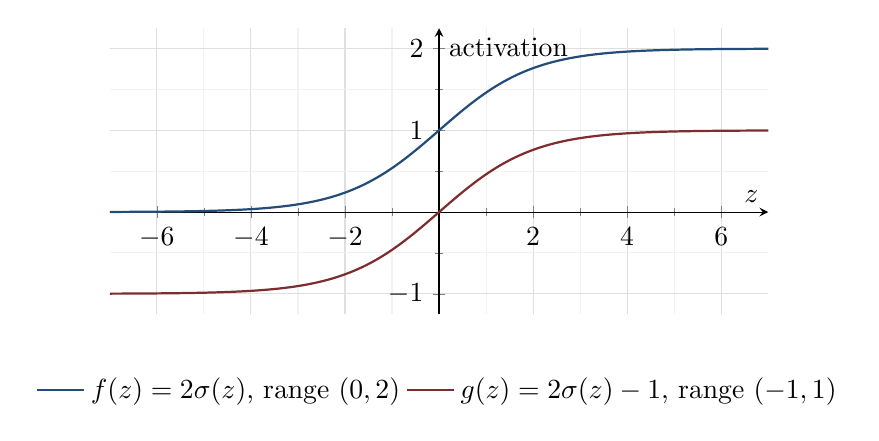
\begin{tikzpicture}
\begin{axis}[
    width=0.82\linewidth,
    height=0.43\linewidth,
    axis lines=middle,
    xmin=-7,xmax=7,
    ymin=-1.25,ymax=2.25,
    xlabel={$z$},ylabel={activation},
    xtick={-6,-4,-2,0,2,4,6},
    ytick={-1,0,1,2},
    legend style={at={(0.5,-0.18)},anchor=north,legend columns=2,draw=none},
    samples=250,
    domain=-7:7,
    grid=both,
    minor tick num=1,
    major grid style={gray!25},
    minor grid style={gray!10}
]
\addplot[thick,deepblue] {2/(1+exp(-x))};
\addlegendentry{$f(z)=2\sigma(z)$, range $(0,2)$}
\addplot[thick,accent] {2/(1+exp(-x))-1};
\addlegendentry{$g(z)=2\sigma(z)-1$, range $(-1,1)$}
\end{axis}
\end{tikzpicture}
\caption{Two activations with identical nonlinear shape and identical derivative, differing only by a vertical translation.}
\label{fig:activations}
\end{figure}

The central question is therefore not one of expressive power: \emph{why can a mere coordinate shift make ordinary gradient descent easier?}

\section{With a following bias, the two activations have the same representational power}

Take one hidden activation \(h\) feeding a downstream affine unit
\begin{equation}
  a=vh+b.
\end{equation}
If the hidden layer uses \(f\), then
\begin{equation}
  a_A=vf(z)+b.
\end{equation}
If it uses \(g=f-1\), then choose a new downstream bias \(\tilde b=b+v\).  The downstream preactivation becomes
\begin{align}
  a_B
  &=v g(z)+\tilde b \\
  &=v(f(z)-1)+(b+v) \\
  &=vf(z)+b \\
  &=a_A.
\end{align}
Thus the two networks compute exactly the same downstream preactivation for every input.

For a vector hidden layer \(h\in\R^m\), let
\[
  \tilde h=h-c\mathbf{1}.
\]
A following affine layer is
\[
  a=Wh+b.
\]
Then
\begin{align}
  W\tilde h+\tilde b
  &=W(h-c\mathbf{1})+\tilde b.
\end{align}
Choosing
\begin{equation}
  \tilde b=b+cW\mathbf{1}
  \label{eq:biasabsorb}
\end{equation}
again gives the identical value \(Wh+b\).

\keybox{\textbf{Representational conclusion.} If a hidden activation is changed only by adding or subtracting a constant, and the following layer has a bias, the constant can be absorbed exactly into that bias.  Therefore centering does not, by itself, enlarge the set of functions the network can represent.  Its advantage is an \emph{optimization} advantage.}

\section{Backpropagation exposes the key sign effect}

This section introduces the one piece of backpropagation notation needed for the zero-centering argument.  The goal is not to give a complete treatment of backpropagation, but to make the sign logic fully explicit.

\subsection{Anatomy of one downstream neuron}

Consider one neuron receiving the hidden activations
\[
  h_1,h_2,\ldots,h_m
\]
from the previous layer.  Collect them into the incoming activation vector
\begin{equation}
  \mathbf h=
  \begin{pmatrix}
    h_1\\ h_2\\ \vdots\\ h_m
  \end{pmatrix}.
\end{equation}
The corresponding incoming weights are
\begin{equation}
  \mathbf w=
  \begin{pmatrix}
    w_1\\ w_2\\ \vdots\\ w_m
  \end{pmatrix}.
\end{equation}
The neuron first forms its preactivation
\begin{equation}
  z=\mathbf w^T\mathbf h+b
   =\sum_{j=1}^{m}w_j h_j+b,
  \label{eq:preactivation}
\end{equation}
and then applies its activation function
\begin{equation}
  y=\phi(z).
\end{equation}
Thus \(h_j\) is simply the activation arriving along the connection whose weight is \(w_j\).

\subsection{The scalar backpropagated error signal \texorpdfstring{\(\delta\)}{delta}}

For one fixed neuron, one fixed training example, and the current parameter values, define
\begin{equation}
  \boxed{\delta\equiv\frac{\partial L}{\partial z}.}
  \label{eq:delta}
\end{equation}
Here \(\delta\) is a \emph{scalar value}: it measures how sensitive the final loss is to a small change in this neuron's preactivation \(z\).

The same scalar \(\delta\) is used for all of the incoming weights of this particular neuron.  It is not, however, a global constant: it generally changes from one training example to another, from one neuron to another, and as the network parameters change during training.

By the chain rule,
\begin{equation}
  \delta
  =\frac{\partial L}{\partial z}
  =\frac{\partial L}{\partial y}\,
    \frac{\partial y}{\partial z}
  =\frac{\partial L}{\partial y}\cdot\phi'(z).
  \label{eq:delta-chain}
\end{equation}
This makes clear why \(\delta\) may be either positive or negative: its sign depends on the downstream loss gradient and on the current network state.

\subsection{Gradient with respect to the incoming weights}

For the scalar weight \(w_j\), the chain rule gives
\begin{align}
  \frac{\partial L}{\partial w_j}
  &=\frac{\partial L}{\partial z}\,
    \frac{\partial z}{\partial w_j} \\
  &=\delta\cdot h_j,
  \label{eq:basicgrad}
\end{align}
because \(\partial z/\partial w_j=h_j\) from \cref{eq:preactivation}.  Likewise,
\begin{equation}
  \frac{\partial L}{\partial b}
  =\frac{\partial L}{\partial z}\,
   \frac{\partial z}{\partial b}
  =\delta\cdot1
  =\delta.
\end{equation}

\keybox{\textbf{Interpretation.} For one incoming connection,
\[
  \underbrace{\frac{\partial L}{\partial w_j}}_{\text{weight gradient}}
  =
  \underbrace{\delta}_{\text{error signal}}
  \cdot
  \underbrace{h_j}_{\text{incoming activation}}.
\]
}

Collecting all incoming-weight derivatives into one vector gives
\begin{equation}
  \boxed{
  \nabla_{\mathbf w}L
  =
  \begin{pmatrix}
    \dfrac{\partial L}{\partial w_1}\\[3pt]
    \dfrac{\partial L}{\partial w_2}\\
    \vdots\\
    \dfrac{\partial L}{\partial w_m}
  \end{pmatrix}
  =\delta\cdot\mathbf h.}
  \label{eq:vectorgrad}
\end{equation}
The notation \(\nabla_{\mathbf w}L\) means the gradient with respect to \emph{all incoming weights of the current neuron}, not with respect to every weight in the entire neural network.

\subsection{Why the sign of the hidden activation matters}

\Cref{eq:vectorgrad} is the heart of the Stanford CS231n intuition.  If the previous hidden layer uses an activation whose output is always positive, such as a logistic sigmoid, then
\[
  h_j>0 \qquad \text{for every }j.
\]
For one training example, the single scalar \(\delta\) therefore determines the sign of every incoming-weight gradient:
\begin{equation}
  \operatorname{sign}\!\left(\frac{\partial L}{\partial w_j}\right)
  =\operatorname{sign}(\delta)
  \qquad \text{for every }j.
  \label{eq:samesign}
\end{equation}
Consequently, all components of \(\nabla_{\mathbf w}L\) are positive when \(\delta>0\), or all are negative when \(\delta<0\).  In two dimensions, the gradient can therefore point only into an all-positive or all-negative quadrant for that example.

If the hidden activations are centered and may take both signs, the products \(\delta\cdot h_j\) need not share a sign.  A single example can immediately produce a mixed-sign gradient such as
\[
  (+,-,+,-,\ldots),
\]
which is impossible when every \(h_j\) is positive.

\subsection{Why \texorpdfstring{\(\delta\)}{delta} itself may be positive or negative}

The fact that a sigmoid output \(y\) is positive does \emph{not} imply that \(\partial L/\partial y\), and hence \(\delta\), must be positive.  For squared error,
\[
  L=\frac12(y-t)^2,
  \qquad
  \frac{\partial L}{\partial y}=y-t.
\]
If \(y=0.3\) and \(t=1\), then \(\partial L/\partial y=-0.7\).  If \(y=0.7\) and \(t=0\), then \(\partial L/\partial y=+0.7\).  Activations describe the current numerical state; gradients describe which infinitesimal direction increases the loss.

For a hidden neuron, the upstream gradient is itself a weighted combination of downstream error signals, so it can again have either sign.  Positivity of the incoming \(h_j\)'s does not fix the sign of \(\delta\); rather, it makes \emph{all incoming-weight gradient components inherit the same sign from that one scalar} for a single example.

\section{The zig-zag phenomenon}

Stanford CS231n makes the sign restriction geometrically intuitive.  Consider only two incoming weights, \(w_1,w_2\), of the current neuron.  With positive hidden inputs \(h_1,h_2>0\), the per-example gradient is
\[
  \nabla_{\mathbf w}L
  =\delta\cdot\mathbf h
  =\delta\cdot
  \begin{pmatrix}h_1\\h_2\end{pmatrix}.
\]
Hence the gradient must have same-sign components.  The gradient-descent update
\[
  \Delta\mathbf w=-\eta\,\nabla_{\mathbf w}L
\]
has the opposite signs, but still has same-sign components; it therefore also lies in one of the same two opposite quadrants.

\begin{figure}[htbp]
\centering
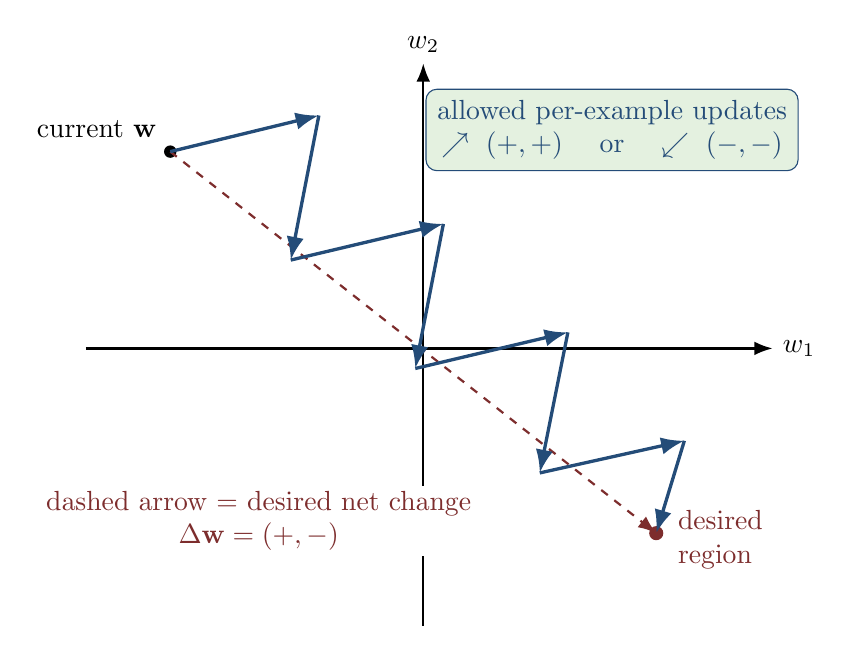
\begin{tikzpicture}[scale=1.02,>=Latex]
  % Parameter-space axes.  The blue arrows below are UPDATE vectors
  % (Delta w = -eta grad L), so each arrow must have same-sign components.
  \draw[->,thick] (-4.2,0)--(4.35,0) node[right] {$w_1$};
  \draw[->,thick] (0,-3.45)--(0,3.55) node[above] {$w_2$};

  % Start, target, and desired mixed-sign net displacement.
  \coordinate (O) at (-3.15,2.45);
  \coordinate (T) at (2.90,-2.30);
  \fill (O) circle (2.2pt) node[above left=2pt] {current $\mathbf w$};
  \fill[accent] (T) circle (2.5pt);
  \node[accent,align=left,anchor=west] at (3.05,-2.38) {desired\\region};
  \draw[dashed,thick,accent,->] (O)--(T);
  \node[accent,align=center,fill=white,inner sep=2pt] at (-2.05,-2.15)
    {dashed arrow = desired net change\\$\Delta\mathbf w=(+,-)$};

  % A deliberately constructed zig-zag.  Every individual displacement
  % is either (+,+) (northeast, quadrant I as a vector) or (-,-)
  % (southwest, quadrant III as a vector).
  \coordinate (P1) at (-1.30,2.90);  % (+,+)
  \coordinate (P2) at (-1.65,1.10);  % (-,-)
  \coordinate (P3) at (0.25,1.55);   % (+,+)
  \coordinate (P4) at (-0.10,-0.25); % (-,-)
  \coordinate (P5) at (1.80,0.20);   % (+,+)
  \coordinate (P6) at (1.45,-1.55);  % (-,-)
  \coordinate (P7) at (3.25,-1.15);  % (+,+)
  \coordinate (P8) at (2.90,-2.30);  % (-,-), target

  \draw[very thick,deepblue,->] (O)--(P1);
  \draw[very thick,deepblue,->] (P1)--(P2);
  \draw[very thick,deepblue,->] (P2)--(P3);
  \draw[very thick,deepblue,->] (P3)--(P4);
  \draw[very thick,deepblue,->] (P4)--(P5);
  \draw[very thick,deepblue,->] (P5)--(P6);
  \draw[very thick,deepblue,->] (P6)--(P7);
  \draw[very thick,deepblue,->] (P7)--(P8);

  % Compact direction key, separated from the trajectory to avoid overlap.
  \node[draw=deepblue,rounded corners,fill=softgreen,align=center,
        inner sep=4pt,text=deepblue] at (2.35,2.72)
        {allowed per-example updates\\
         $\nearrow\ (+,+)$ \quad or \quad $\swarrow\ (-,-)$};
\end{tikzpicture}
\caption{Corrected schematic of the CS231n ``zig-zag'' intuition.  The blue arrows are gradient-descent updates, $\Delta\mathbf w=-\eta\nabla_{\mathbf w} L$.  Every individual blue arrow has same-sign components---it points northeast $(+,+)$ or southwest $(-,-)$ relative to its own tail.  Nevertheless, alternating such steps can accumulate to the mixed-sign net displacement indicated by the dashed red arrow.  The picture is illustrative, not a literal trajectory for every loss surface.}
\label{fig:zigzag}
\end{figure}

Suppose the optimization would benefit from increasing \(w_1\) while decreasing \(w_2\).  That is a mixed-sign displacement.  A single-example update generated from strictly positive inputs cannot point directly in that direction.  Across successive examples, the scalar \(\delta\) may change sign; alternating same-sign steps can then produce a mixed-sign \emph{net} displacement, but the path can zig-zag rather than move directly.

This argument should be interpreted carefully:
\begin{itemize}
  \item It is sharpest for a \emph{single training example} or stochastic-gradient step.
  \item With a minibatch, gradients are sums
  \[
    \frac{\partial L}{\partial w_j}=\sum_i \delta_i\cdot h_{ij},
  \]
  and different examples can partially cancel.  Stanford explicitly notes that minibatches help.
  \item The argument is an optimization heuristic, not a proof that every positive activation causes slow training.
\end{itemize}

Nevertheless, it cleanly explains why translating an otherwise identical activation from \((0,2)\) to \((-1,1)\) can change the geometry of SGD updates even though the network's representational power is unchanged.

\section{A second intuition: zero mean separates ``baseline'' from ``variation''}

The sign argument is local and per-example.  A complementary viewpoint appears when one asks how the mean of a hidden feature interacts with the next layer's bias.

Write a scalar hidden feature as
\begin{equation}
  h=\mu+\tilde h,
  \qquad
  \E[\tilde h]=0.
\end{equation}
A downstream affine model is
\begin{align}
  a&=wh+b\\
   &=w(\mu+\tilde h)+b\\
   &=w\tilde h+(b+w\mu).
  \label{eq:effectivebias}
\end{align}
If \(\mu\neq0\), changing \(w\) also changes the effective baseline \(b+w\mu\).  Thus the weight has two intertwined roles:
\begin{enumerate}
  \item responding to variation \(\tilde h\), and
  \item shifting the baseline through \(w\mu\).
\end{enumerate}
If \(\mu=0\), these roles are naturally separated: \(w\) controls sensitivity to the centered feature and \(b\) controls the baseline.

This is why the useful property is more precisely
\begin{equation}
  \boxed{\E[h]\approx0,}
\end{equation}
not merely ``the mathematical range includes negative numbers.''  A function with range \((-1,1)\) can still produce activations with mean \(0.8\) if most preactivations lie on its positive side.

\section{Advanced / Optional: The Hessian view}

\keybox{\textbf{Advanced / optional section.} The main zero-centering argument does not require Hessians.  This section gives a more formal curvature/conditioning interpretation for readers who want the optimization mathematics.  It may be skipped without affecting the later practical conclusions.}

The previous intuition can be made exact in a simple model.  Consider
\begin{equation}
  \hat y=wh+b
\end{equation}
with squared loss
\begin{equation}
  L=\frac12(\hat y-y)^2.
\end{equation}
For one observation, the second-derivative matrix with respect to \((w,b)\) is
\[
  \begin{pmatrix}
    h^2 & h\\
    h & 1
  \end{pmatrix}.
\]
Averaging over the data gives
\begin{equation}
  \boxed{
  H=
  \begin{pmatrix}
    \E[h^2] & \E[h]\\
    \E[h] & 1
  \end{pmatrix}.}
  \label{eq:hessian}
\end{equation}
The off-diagonal term is exactly \(\E[h]\).  If the feature is centered,
\begin{equation}
  \E[h]=0,
\end{equation}
then
\begin{equation}
  H=
  \begin{pmatrix}
    \E[h^2] & 0\\
    0 & 1
  \end{pmatrix},
\end{equation}
and the weight and bias directions are locally decoupled in this model.

For a vector hidden representation \(h\in\R^m\), the same structure becomes
\begin{equation}
  H=
  \begin{pmatrix}
    \E[hh^T] & \E[h]\\
    \E[h]^T & 1
  \end{pmatrix}.
  \label{eq:vectorhessian}
\end{equation}
Centering makes the weight--bias cross block vanish.  It does \emph{not} automatically decorrelate the hidden features from each other; the matrix \(\E[hh^T]\) can still have substantial off-diagonal terms.  Thus centering is useful but not equivalent to full whitening.

\subsection{A numerical example}

Let the uncentered hidden values be
\[
  h\in\{0.5,1.5\}
\]
with equal probability.  Then
\[
  \E[h]=1,
  \qquad
  \E[h^2]=1.25,
\]
so
\[
  H_{\mathrm{uncentered}}=
  \begin{pmatrix}
    1.25&1\\
    1&1
  \end{pmatrix}.
\]
Now center the same information:
\[
  \tilde h=h-1\in\{-0.5,+0.5\}.
\]
Then
\[
  \E[\tilde h]=0,
  \qquad
  \E[\tilde h^2]=0.25,
\]
so
\[
  H_{\mathrm{centered}}=
  \begin{pmatrix}
    0.25&0\\
    0&1
  \end{pmatrix}.
\]
The centered parameterization has removed the cross-term completely.  In this example the approximate spectral condition number falls from about \(18.2\) to \(4\), illustrating why the corresponding quadratic loss can be easier for first-order gradient descent.

\keybox{\textbf{Connection between the two explanations.} The Stanford zig-zag picture emphasizes per-example gradient signs.  The Hessian argument emphasizes parameter coupling and conditioning over a data distribution.  They are not identical arguments, but both arise because a nonzero activation mean makes downstream weight coordinates interact with the baseline.}

\section{Why random initialization strengthens the case for centering}

Assume a conventional random initialization in which weights are drawn from a distribution symmetric about zero and initial biases are near zero.  Early in training, preactivations are therefore often approximately symmetric around zero.

For the centered activation
\begin{equation}
  g(z)=2\sigma(z)-1,
\end{equation}
we have the odd-symmetry property
\begin{equation}
  g(-z)=-g(z).
\end{equation}
If the distribution of \(z\) is symmetric, this implies
\begin{equation}
  \E[g(z)]=0.
\end{equation}
For the shifted activation
\[
  f(z)=g(z)+1,
\]
we instead get
\begin{equation}
  \E[f(z)]=1.
\end{equation}
Thus, under the same initialization, the centered version naturally sends an approximately zero-mean signal to the next layer.

The difference can also be seen directly in the next preactivation.  Let
\[
  h=\mathbf{1}+\tilde h,
  \qquad \E[\tilde h]\approx0.
\]
Then
\begin{equation}
  z_{\text{next}}=W h+b
  =W\tilde h+W\mathbf{1}+b.
  \label{eq:randomoffset}
\end{equation}
The term \(W\mathbf{1}\) acts like an additional random offset.  Across random initializations its expectation may be zero, but in any one initialized network it is generally nonzero.  Centering removes this particular offset term.

This observation aligns with the historical analysis of Glorot and Bengio, who found that the nonzero mean of logistic-sigmoid activations is problematic in deep networks under random initialization and can contribute to saturation of upper layers \cite{glorot2010}.

\section{Why this is a preference, not a universal law}

Zero-centered hidden activations are often a better default in the narrow comparison considered here, but several qualifications matter.

\subsection{Saturation can dominate centering}

Both logistic sigmoid and tanh saturate.  Their derivatives approach zero in the tails.  A centered saturating activation may still train worse than a non-centered activation that avoids saturation.  ReLU is the classic counterexample: it is not zero-centered, yet its positive branch has derivative one and historically proved much easier to optimize in many deep architectures.

\subsection{Range does not guarantee empirical centering}

A function with range \((-1,1)\) is not automatically zero-mean in actual use.  If most preactivations are positive, then its empirical activation mean may also be strongly positive.

\subsection{Normalization can change the comparison}

If a network explicitly normalizes internal representations, then the natural centering advantage of a \((-1,1)\) activation may be reduced or partly replaced by the normalization mechanism.  BatchNorm and LayerNorm explicitly subtract a mean; RMSNorm, notably, does not.  These methods are summarized in \cref{app:norm}.

\subsection{Output layers have different semantics}

For binary classification, a logistic sigmoid is useful precisely because its output lies in \((0,1)\) and can be interpreted as a Bernoulli probability.  The zero-centering argument is primarily about \emph{hidden representations}, not a rule that all network outputs should be centered.

\section{Practical rule of thumb}

For two otherwise equivalent monotone S-shaped hidden activations that differ mainly by a constant vertical shift, under ordinary random initialization, with downstream biases and without normalization, the centered version is generally the preferable default.

A useful summary is:
\begin{equation}
\boxed{
\begin{gathered}
\bigl(\text{same function class}\bigr)
\;\land\;
\bigl(\text{same derivative shape}\bigr)\\[-1pt]
\land\;\bigl(\text{following-layer bias}\bigr)\\[4pt]
\Downarrow\\[-1pt]
\text{centering changes optimization geometry, not expressivity}
\end{gathered}}
\end{equation}

The most important benefits are:
\begin{itemize}
  \item per-example gradients are not forced into only same-sign weight directions;
  \item the bias can represent the baseline while weights represent deviations around it;
  \item the weight--bias cross-coupling term disappears in the simple Hessian model when \(\E[h]=0\);
  \item symmetric random initialization naturally produces approximately zero-mean activations for an odd centered nonlinearity.
\end{itemize}

\section{Recommended educational sources}

The following sources complement one another rather than replacing one another.

\begin{enumerate}
  \item \textbf{Stanford CS231n, Lecture 7: Training Neural Networks} \cite{cs231n2023}.  Slides 29--33 give the clearest short visual explanation of the same-sign gradient restriction and the resulting zig-zag path, followed immediately by the observation that tanh is zero-centered.

  \item \textbf{LeCun, Bottou, Orr, and M\"uller, ``Efficient BackProp''} \cite{lecun1998}.  This is the strongest classical educational source for the broader optimization argument: centering, scaling, curvature, and convergence of backpropagation.

  \item \textbf{Glorot and Bengio, 2010} \cite{glorot2010}.  This paper directly studies random initialization in deep feed-forward networks and explicitly identifies the nonzero mean of logistic-sigmoid activations as problematic.

  \item \textbf{Goodfellow, Bengio, and Courville, \emph{Deep Learning}} \cite{goodfellow2016}.  Chapters on numerical optimization and training deep models provide the broader language of ill-conditioning, curvature, initialization, and gradient propagation.
\end{enumerate}

\appendix

\section{Subdivision-based and spline-based saturating activation functions}
\label{app:subdivision}

The preceding discussion concerns centering, but it also motivates a broader question: must a sigmoid-like activation be an exponential function such as logistic sigmoid or tanh?  No.  Many monotone saturating curves can serve as nonlinear activations, although their optimization properties can differ substantially.

\subsection{From corner cutting to smooth transitions}

Chaikin's corner-cutting algorithm repeatedly replaces a control polygon by a refined polygon obtained by cutting corners.  The classical Chaikin scheme converges to a quadratic B-spline curve \cite{chaikin1974,caltechchaikin}.  This makes the following construction conceptually natural: begin with a step-like or clipped control shape, apply a subdivision rule, and obtain a smooth or piecewise-smooth saturating transition.

One should distinguish this intuition from a specific neural-network result.  The 2024 work of L\'opez-Ure\~na does not merely say ``apply Chaikin to a step.''  It develops activation functions from the limit functions of convergent subdivision schemes and requires two structural properties: \emph{refinability} and the ability to \emph{sum the identity} \cite{lopezurena2024}.  These properties permit function-preserving widening and deepening of a neural network.

\subsection{A quadratic spline activation}

A representative centered spline activation presented by L\'opez-Ure\~na is
\begin{equation}
\sigma_{B^2}(t)=
\begin{cases}
-\frac12, & t\le -1,\\[4pt]
 t\left(1-\frac{|t|}{2}\right), & -1\le t\le 1,\\[4pt]
 \frac12, & t\ge 1.
\end{cases}
\label{eq:splineact}
\end{equation}
It is monotone and saturating, but unlike logistic sigmoid or tanh it reaches exact saturation at finite \(|t|\).

Its derivative is especially simple:
\begin{equation}
\sigma_{B^2}'(t)=
\begin{cases}
0, & |t|\ge1,\\[3pt]
1-|t|, & |t|<1.
\end{cases}
\label{eq:splinederiv}
\end{equation}
Thus the derivative is triangular.  This is computationally simple, but exact saturation means that a neuron outside the transition interval has an exactly zero local derivative rather than merely a very small one.

\begin{figure}[htbp]
\centering
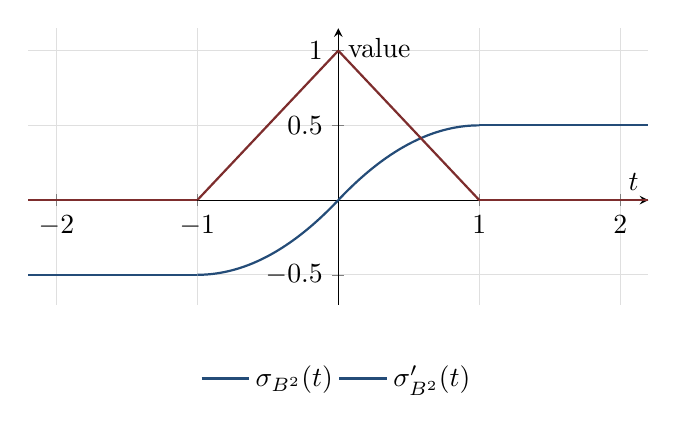
\begin{tikzpicture}
\begin{axis}[
  width=0.78\linewidth,height=0.42\linewidth,
  axis lines=middle,xmin=-2.2,xmax=2.2,ymin=-0.7,ymax=1.15,
  xlabel={$t$},ylabel={value},
  xtick={-2,-1,0,1,2},ytick={-0.5,0,0.5,1},
  legend style={at={(0.5,-0.18)},anchor=north,legend columns=2,draw=none},
  samples=100,
  grid=both,major grid style={gray!25},minor grid style={gray!10}
]
\addplot[thick,deepblue,domain=-2.2:-1] {-0.5};
\addplot[thick,deepblue,domain=-1:0] {x*(1+x/2)};
\addplot[thick,deepblue,domain=0:1] {x*(1-x/2)};
\addplot[thick,deepblue,domain=1:2.2] {0.5};
\addlegendentry{$\sigma_{B^2}(t)$}
\addplot[thick,accent,domain=-2.2:-1] {0};
\addplot[thick,accent,domain=-1:0] {1+x};
\addplot[thick,accent,domain=0:1] {1-x};
\addplot[thick,accent,domain=1:2.2] {0};
\addlegendentry{$\sigma_{B^2}'(t)$}
\end{axis}
\end{tikzpicture}
\caption{A subdivision-derived quadratic spline activation and its triangular derivative.}
\label{fig:spline}
\end{figure}

\subsection{Why ``without altering outcomes'' matters}

The same paper studies activations satisfying a refinement identity of the form
\begin{equation}
  \sigma(t)=\sum_{\ell=0}^{A-1} a_\ell\,\sigma(2t+\tau-\ell),
\end{equation}
which allows one neuron to be replaced by several scaled and shifted copies while preserving the function computed by the network.  A second identity lets collections of activations sum to the identity map over an interval, allowing insertion of a new nonlinear layer without initially changing the network output \cite{lopezurena2024}.

The purpose is therefore not simply to invent another S-shaped curve.  The subdivision structure provides algebraic identities that can preserve a trained function while the architecture is widened or deepened.  After the transformation, training can continue in a larger parameter space.

\section{Normalization layers and their relation to centering}
\label{app:norm}

Modern deep networks frequently control internal signal statistics explicitly.  This reduces the extent to which an activation function must provide centering by itself.

\subsection{Batch Normalization}

Batch Normalization (BatchNorm) normalizes a feature using statistics computed across a minibatch \cite{ioffe2015}:
\begin{equation}
  \hat z=\frac{z-\mu_{\mathrm{batch}}}{\sqrt{\sigma^2_{\mathrm{batch}}+\epsilon}},
  \qquad
  y=\gamma\hat z+\beta.
\end{equation}
It explicitly recenters and rescales the signal, then restores learnable scale and offset through \(\gamma\) and \(\beta\).  Its drawbacks include dependence on batch statistics, sensitivity to small batches, and a distinction between training-time and inference-time behavior.

\subsection{Layer Normalization}

Layer Normalization (LayerNorm) computes mean and variance across features of a single example rather than across a minibatch \cite{ba2016}:
\begin{equation}
  \hat z_j=\frac{z_j-\mu_{\mathrm{layer}}}{\sqrt{\sigma^2_{\mathrm{layer}}+\epsilon}},
  \qquad
  y_j=\gamma_j\hat z_j+\beta_j.
\end{equation}
It therefore does not depend on which other examples happen to be in the minibatch and performs the same basic normalization at training and inference time.

\subsection{RMSNorm: an important qualification to the centering story}

RMSNorm deliberately removes the mean-subtraction step and normalizes primarily by root-mean-square magnitude \cite{zhang2019}:
\begin{equation}
  \operatorname{RMS}(z)=\sqrt{\frac{1}{m}\sum_{j=1}^{m}z_j^2+\epsilon},
  \qquad
  y_j=\gamma_j\frac{z_j}{\operatorname{RMS}(z)}.
\end{equation}
The success of RMSNorm is an important caution against overgeneralizing the slogan ``zero mean is always necessary.''  Re-centering is often useful, but modern optimization also depends critically on controlling scale, residual pathways, initialization, and the architecture as a whole.

\subsection{What normalization changes in the \((0,2)\) vs. \((-1,1)\) comparison}

If a normalization layer explicitly subtracts the mean after a hidden transformation, then much of the natural centering advantage of a \((-1,1)\) activation can disappear.  In a plain multilayer perceptron without normalization, activation centering directly changes the signal received by the next layer.  In a normalized architecture, that signal may be recentered or rescaled before the next transformation.

This is why the classical tanh-versus-sigmoid centering discussion is most transparent in unnormalized feed-forward networks.  Modern architectures still care deeply about conditioning and stable signal propagation, but they may achieve those goals using normalization, residual connections, careful initialization, or combinations of these techniques rather than relying on the activation function alone.

\begin{thebibliography}{99}

\bibitem{cs231n2023}
F.-F. Li, Y. Li, and R. Gao,
\emph{CS231n: Deep Learning for Computer Vision, Lecture 7: Training Neural Networks},
Stanford University, April 25, 2023.
\url{https://cs231n.stanford.edu/slides/2023/lecture_7.pdf}.

\bibitem{lecun1998}
Y. LeCun, L. Bottou, G. B. Orr, and K.-R. M\"uller,
``Efficient BackProp,''
in \emph{Neural Networks: Tricks of the Trade},
Lecture Notes in Computer Science, vol. 1524, Springer, 1998.
\url{https://leon.bottou.org/papers/lecun-98x}.

\bibitem{glorot2010}
X. Glorot and Y. Bengio,
``Understanding the difficulty of training deep feedforward neural networks,''
in \emph{Proceedings of the Thirteenth International Conference on Artificial Intelligence and Statistics (AISTATS)},
PMLR 9:249--256, 2010.
\url{https://proceedings.mlr.press/v9/glorot10a.html}.

\bibitem{goodfellow2016}
I. Goodfellow, Y. Bengio, and A. Courville,
\emph{Deep Learning}.
MIT Press, 2016.
\url{https://www.deeplearningbook.org/}.

\bibitem{lopezurena2024}
S. L\'opez-Ure\~na,
``Activation functions enabling the addition of neurons and layers without altering outcomes,''
arXiv:2410.12625, first posted 2024; revised version 2025.
\url{https://arxiv.org/abs/2410.12625}.

\bibitem{chaikin1974}
G. M. Chaikin,
``An algorithm for high speed curve generation,''
\emph{Computer Graphics and Image Processing}, vol. 3, pp. 346--349, 1974.

\bibitem{caltechchaikin}
Caltech Multi-Res Modeling Group,
``Chaikin's Algorithm: Drawing Smooth Curves through Corner Cutting.''
\url{https://multires.caltech.edu/teaching/demos/java/chaikin.htm}.

\bibitem{ioffe2015}
S. Ioffe and C. Szegedy,
``Batch Normalization: Accelerating Deep Network Training by Reducing Internal Covariate Shift,''
arXiv:1502.03167, 2015.
\url{https://arxiv.org/abs/1502.03167}.

\bibitem{ba2016}
J. L. Ba, J. R. Kiros, and G. E. Hinton,
``Layer Normalization,''
arXiv:1607.06450, 2016.
\url{https://arxiv.org/abs/1607.06450}.

\bibitem{zhang2019}
B. Zhang and R. Sennrich,
``Root Mean Square Layer Normalization,''
arXiv:1910.07467, 2019.
\url{https://arxiv.org/abs/1910.07467}.

\end{thebibliography}

\end{document}
